%% bare_jrnl.tex
%% V1.4b
%% 2015/08/26
%% by Michael Shell
%% see http://www.michaelshell.org/
%% for current contact information.
%%
%% This is a skeleton file demonstrating the use of IEEEtran.cls
%% (requires IEEEtran.cls version 1.8b or later) with an IEEE
%% journal paper.
%%
%% Support sites:
%% http://www.michaelshell.org/tex/ieeetran/
%% http://www.ctan.org/pkg/ieeetran
%% and
%% http://www.ieee.org/

%%*************************************************************************
%% Legal Notice:
%% This code is offered as-is without any warranty either expressed or
%% implied; without even the implied warranty of MERCHANTABILITY or
%% FITNESS FOR A PARTICULAR PURPOSE! 
%% User assumes all risk.
%% In no event shall the IEEE or any contributor to this code be liable for
%% any damages or losses, including, but not limited to, incidental,
%% consequential, or any other damages, resulting from the use or misuse
%% of any information contained here.
%%
%% All comments are the opinions of their respective authors and are not
%% necessarily endorsed by the IEEE.
%%
%% This work is distributed under the LaTeX Project Public License (LPPL)
%% ( http://www.latex-project.org/ ) version 1.3, and may be freely used,
%% distributed and modified. A copy of the LPPL, version 1.3, is included
%% in the base LaTeX documentation of all distributions of LaTeX released
%% 2003/12/01 or later.
%% Retain all contribution notices and credits.
%% ** Modified files should be clearly indicated as such, including  **
%% ** renaming them and changing author support contact information. **
%%*************************************************************************


% *** Authors should verify (and, if needed, correct) their LaTeX system  ***
% *** with the testflow diagnostic prior to trusting their LaTeX platform ***
% *** with production work. The IEEE's font choices and paper sizes can   ***
% *** trigger bugs that do not appear when using other class files.       ***                          ***
% The testflow support page is at:
% http://www.michaelshell.org/tex/testflow/


% Please refer to your journal's instructions for other
% options that should be set.
\documentclass[journal,onecolumn]{IEEEtran}
%
% If IEEEtran.cls has not been installed into the LaTeX system files,
% manually specify the path to it like:
% \documentclass[journal]{../sty/IEEEtran}





% Some very useful LaTeX packages include:
% (uncomment the ones you want to load)


% *** MISC UTILITY PACKAGES ***
%
%\usepackage{ifpdf}
% Heiko Oberdiek's ifpdf.sty is very useful if you need conditional
% compilation based on whether the output is pdf or dvi.
% usage:
% \ifpdf
%   % pdf code
% \else
%   % dvi code
% \fi
% The latest version of ifpdf.sty can be obtained from:
% http://www.ctan.org/pkg/ifpdf
% Also, note that IEEEtran.cls V1.7 and later provides a builtin
% \ifCLASSINFOpdf conditional that works the same way.
% When switching from latex to pdflatex and vice-versa, the compiler may
% have to be run twice to clear warning/error messages.



\usepackage{caption}
\usepackage{subcaption}
\usepackage[bottom]{footmisc}


% *** CITATION PACKAGES ***
%
\usepackage{cite}
% cite.sty was written by Donald Arseneau
% V1.6 and later of IEEEtran pre-defines the format of the cite.sty package
% \cite{} output to follow that of the IEEE. Loading the cite package will
% result in citation numbers being automatically sorted and properly
% "compressed/ranged". e.g., [1], [9], [2], [7], [5], [6] without using
% cite.sty will become [1], [2], [5]--[7], [9] using cite.sty. cite.sty's
% \cite will automatically add leading space, if needed. Use cite.sty's
% noadjust option (cite.sty V3.8 and later) if you want to turn this off
% such as if a citation ever needs to be enclosed in parenthesis.
% cite.sty is already installed on most LaTeX systems. Be sure and use
% version 5.0 (2009-03-20) and later if using hyperref.sty.
% The latest version can be obtained at:
% http://www.ctan.org/pkg/cite
% The documentation is contained in the cite.sty file itself.
\usepackage{booktabs}
\usepackage{multirow}
\usepackage[table,xcdraw]{xcolor}





% *** GRAPHICS RELATED PACKAGES ***
%
\ifCLASSINFOpdf
  \usepackage[pdftex]{graphicx}
  % declare the path(s) where your graphic files are
  \graphicspath{/figures}
  % and their extensions so you won't have to specify these with
  % every instance of \includegraphics
  \DeclareGraphicsExtensions{.pdf,.jpeg,.png}
\else
  % or other class option (dvipsone, dvipdf, if not using dvips). graphicx
  % will default to the driver specified in the system graphics.cfg if no
  % driver is specified.
  % \usepackage[dvips]{graphicx}
  % declare the path(s) where your graphic files are
  % \graphicspath{{../eps/}}
  % and their extensions so you won't have to specify these with
  % every instance of \includegraphics
  % \DeclareGraphicsExtensions{.eps}
\fi
% graphicx was written by David Carlisle and Sebastian Rahtz. It is
% required if you want graphics, photos, etc. graphicx.sty is already
% installed on most LaTeX systems. The latest version and documentation
% can be obtained at: 
% http://www.ctan.org/pkg/graphicx
% Another good source of documentation is "Using Imported Graphics in
% LaTeX2e" by Keith Reckdahl which can be found at:
% http://www.ctan.org/pkg/epslatex
%
% latex, and pdflatex in dvi mode, support graphics in encapsulated
% postscript (.eps) format. pdflatex in pdf mode supports graphics
% in .pdf, .jpeg, .png and .mps (metapost) formats. Users should ensure
% that all non-photo figures use a vector format (.eps, .pdf, .mps) and
% not a bitmapped formats (.jpeg, .png). The IEEE frowns on bitmapped formats
% which can result in "jaggedy"/blurry rendering of lines and letters as
% well as large increases in file sizes.
%
% You can find documentation about the pdfTeX application at:
% http://www.tug.org/applications/pdftex





% *** MATH PACKAGES ***
%
\usepackage{amsmath}
% A popular package from the American Mathematical Society that provides
% many useful and powerful commands for dealing with mathematics.
%
% Note that the amsmath package sets \interdisplaylinepenalty to 10000
% thus preventing page breaks from occurring within multiline equations. Use:
\interdisplaylinepenalty=2500
% after loading amsmath to restore such page breaks as IEEEtran.cls normally
% does. amsmath.sty is already installed on most LaTeX systems. The latest
% version and documentation can be obtained at:
% http://www.ctan.org/pkg/amsmath





% *** SPECIALIZED LIST PACKAGES ***
%
%\usepackage{algorithmic}
% algorithmic.sty was written by Peter Williams and Rogerio Brito.
% This package provides an algorithmic environment fo describing algorithms.
% You can use the algorithmic environment in-text or within a figure
% environment to provide for a floating algorithm. Do NOT use the algorithm
% floating environment provided by algorithm.sty (by the same authors) or
% algorithm2e.sty (by Christophe Fiorio) as the IEEE does not use dedicated
% algorithm float types and packages that provide these will not provide
% correct IEEE style captions. The latest version and documentation of
% algorithmic.sty can be obtained at:
% http://www.ctan.org/pkg/algorithms
% Also of interest may be the (relatively newer and more customizable)
% algorithmicx.sty package by Szasz Janos:
% http://www.ctan.org/pkg/algorithmicx




% *** ALIGNMENT PACKAGES ***
%
%\usepackage{array}
% Frank Mittelbach's and David Carlisle's array.sty patches and improves
% the standard LaTeX2e array and tabular environments to provide better
% appearance and additional user controls. As the default LaTeX2e table
% generation code is lacking to the point of almost being broken with
% respect to the quality of the end results, all users are strongly
% advised to use an enhanced (at the very least that provided by array.sty)
% set of table tools. array.sty is already installed on most systems. The
% latest version and documentation can be obtained at:
% http://www.ctan.org/pkg/array


% IEEEtran contains the IEEEeqnarray family of commands that can be used to
% generate multiline equations as well as matrices, tables, etc., of high
% quality.




% *** SUBFIGURE PACKAGES ***
%\ifCLASSOPTIONcompsoc
%  \usepackage[caption=false,font=normalsize,labelfont=sf,textfont=sf]{subfig}
%\else
%  \usepackage[caption=false,font=footnotesize]{subfig}
%\fi
% subfig.sty, written by Steven Douglas Cochran, is the modern replacement
% for subfigure.sty, the latter of which is no longer maintained and is
% incompatible with some LaTeX packages including fixltx2e. However,
% subfig.sty requires and automatically loads Axel Sommerfeldt's caption.sty
% which will override IEEEtran.cls' handling of captions and this will result
% in non-IEEE style figure/table captions. To prevent this problem, be sure
% and invoke subfig.sty's "caption=false" package option (available since
% subfig.sty version 1.3, 2005/06/28) as this is will preserve IEEEtran.cls
% handling of captions.
% Note that the Computer Society format requires a larger sans serif font
% than the serif footnote size font used in traditional IEEE formatting
% and thus the need to invoke different subfig.sty package options depending
% on whether compsoc mode has been enabled.
%
% The latest version and documentation of subfig.sty can be obtained at:
% http://www.ctan.org/pkg/subfig




% *** FLOAT PACKAGES ***
%
%\usepackage{fixltx2e}
% fixltx2e, the successor to the earlier fix2col.sty, was written by
% Frank Mittelbach and David Carlisle. This package corrects a few problems
% in the LaTeX2e kernel, the most notable of which is that in current
% LaTeX2e releases, the ordering of single and double column floats is not
% guaranteed to be preserved. Thus, an unpatched LaTeX2e can allow a
% single column figure to be placed prior to an earlier double column
% figure.
% Be aware that LaTeX2e kernels dated 2015 and later have fixltx2e.sty's
% corrections already built into the system in which case a warning will
% be issued if an attempt is made to load fixltx2e.sty as it is no longer
% needed.
% The latest version and documentation can be found at:
% http://www.ctan.org/pkg/fixltx2e


%\usepackage{stfloats}
% stfloats.sty was written by Sigitas Tolusis. This package gives LaTeX2e
% the ability to do double column floats at the bottom of the page as well
% as the top. (e.g., "\begin{figure*}[!b]" is not normally possible in
% LaTeX2e). It also provides a command:
%\fnbelowfloat
% to enable the placement of footnotes below bottom floats (the standard
% LaTeX2e kernel puts them above bottom floats). This is an invasive package
% which rewrites many portions of the LaTeX2e float routines. It may not work
% with other packages that modify the LaTeX2e float routines. The latest
% version and documentation can be obtained at:
% http://www.ctan.org/pkg/stfloats
% Do not use the stfloats baselinefloat ability as the IEEE does not allow
% \baselineskip to stretch. Authors submitting work to the IEEE should note
% that the IEEE rarely uses double column equations and that authors should try
% to avoid such use. Do not be tempted to use the cuted.sty or midfloat.sty
% packages (also by Sigitas Tolusis) as the IEEE does not format its papers in
% such ways.
% Do not attempt to use stfloats with fixltx2e as they are incompatible.
% Instead, use Morten Hogholm'a dblfloatfix which combines the features
% of both fixltx2e and stfloats:
%
% \usepackage{dblfloatfix}
% The latest version can be found at:
% http://www.ctan.org/pkg/dblfloatfix




%\ifCLASSOPTIONcaptionsoff
%  \usepackage[nomarkers]{endfloat}
% \let\MYoriglatexcaption\caption
% \renewcommand{\caption}[2][\relax]{\MYoriglatexcaption[#2]{#2}}
%\fi
% endfloat.sty was written by James Darrell McCauley, Jeff Goldberg and 
% Axel Sommerfeldt. This package may be useful when used in conjunction with 
% IEEEtran.cls'  captionsoff option. Some IEEE journals/societies require that
% submissions have lists of figures/tables at the end of the paper and that
% figures/tables without any captions are placed on a page by themselves at
% the end of the document. If needed, the draftcls IEEEtran class option or
% \CLASSINPUTbaselinestretch interface can be used to increase the line
% spacing as well. Be sure and use the nomarkers option of endfloat to
% prevent endfloat from "marking" where the figures would have been placed
% in the text. The two hack lines of code above are a slight modification of
% that suggested by in the endfloat docs (section 8.4.1) to ensure that
% the full captions always appear in the list of figures/tables - even if
% the user used the short optional argument of \caption[]{}.
% IEEE papers do not typically make use of \caption[]'s optional argument,
% so this should not be an issue. A similar trick can be used to disable
% captions of packages such as subfig.sty that lack options to turn off
% the subcaptions:
% For subfig.sty:
% \let\MYorigsubfloat\subfloat
% \renewcommand{\subfloat}[2][\relax]{\MYorigsubfloat[]{#2}}
% However, the above trick will not work if both optional arguments of
% the \subfloat command are used. Furthermore, there needs to be a
% description of each subfigure *somewhere* and endfloat does not add
% subfigure captions to its list of figures. Thus, the best approach is to
% avoid the use of subfigure captions (many IEEE journals avoid them anyway)
% and instead reference/explain all the subfigures within the main caption.
% The latest version of endfloat.sty and its documentation can obtained at:
% http://www.ctan.org/pkg/endfloat
%
% The IEEEtran \ifCLASSOPTIONcaptionsoff conditional can also be used
% later in the document, say, to conditionally put the References on a 
% page by themselves.




% *** PDF, URL AND HYPERLINK PACKAGES ***
%
%\usepackage{url}
% url.sty was written by Donald Arseneau. It provides better support for
% handling and breaking URLs. url.sty is already installed on most LaTeX
% systems. The latest version and documentation can be obtained at:
% http://www.ctan.org/pkg/url
% Basically, \url{my_url_here}.




% *** Do not adjust lengths that control margins, column widths, etc. ***
% *** Do not use packages that alter fonts (such as pslatex).         ***
% There should be no need to do such things with IEEEtran.cls V1.6 and later.
% (Unless specifically asked to do so by the journal or conference you plan
% to submit to, of course. )


% correct bad hyphenation here
\hyphenation{op-tical net-works semi-conduc-tor}


\begin{document}
%
% paper title
% Titles are generally capitalized except for words such as a, an, and, as,
% at, but, by, for, in, nor, of, on, or, the, to and up, which are usually
% not capitalized unless they are the first or last word of the title.
% Linebreaks \\ can be used within to get better formatting as desired.
% Do not put math or special symbols in the title.
\title{Linguistic Steganography Using a Transformer-based Causal Language Model}
%
%
% author names and IEEE memberships
% note positions of commas and nonbreaking spaces ( ~ ) LaTeX will not break
% a structure at a ~ so this keeps an author's name from being broken across
% two lines.
% use \thanks{} to gain access to the first footnote area
% a separate \thanks must be used for each paragraph as LaTeX2e's \thanks
% was not built to handle multiple paragraphs
%

\author{Arian~Tashakkor,~\IEEEmembership{40023494}\\Shahab~Mohrehkesh,~\IEEEmembership{40032134}}

% note the % following the last \IEEEmembership and also \thanks - 
% these prevent an unwanted space from occurring between the last author name
% and the end of the author line. i.e., if you had this:
% 
% \author{....lastname \thanks{...} \thanks{...} }
%                     ^------------^------------^----Do not want these spaces!
%
% a space would be appended to the last name and could cause every name on that
% line to be shifted left slightly. This is one of those "LaTeX things". For
% instance, "\textbf{A} \textbf{B}" will typeset as "A B" not "AB". To get
% "AB" then you have to do: "\textbf{A}\textbf{B}"
% \thanks is no different in this regard, so shield the last } of each \thanks
% that ends a line with a % and do not let a space in before the next \thanks.
% Spaces after \IEEEmembership other than the last one are OK (and needed) as
% you are supposed to have spaces between the names. For what it is worth,
% this is a minor point as most people would not even notice if the said evil
% space somehow managed to creep in.



% The paper headers
% The only time the second header will appear is for the odd numbered pages
% after the title page when using the twoside option.
% 
% *** Note that you probably will NOT want to include the author's ***
% *** name in the headers of peer review papers.                   ***
% You can use \ifCLASSOPTIONpeerreview for conditional compilation here if
% you desire.




% If you want to put a publisher's ID mark on the page you can do it like
% this:
%\IEEEpubid{0000--0000/00\$00.00~\copyright~2015 IEEE}
% Remember, if you use this you must call \IEEEpubidadjcol in the second
% column for its text to clear the IEEEpubid mark.



% use for special paper notices
%\IEEEspecialpapernotice{(Invited Paper)}




% make the title area
\maketitle

% As a general rule, do not put math, special symbols or citations
% in the abstract or keywords.
\begin{abstract}
This is the report for the final project of the Advanced Information Retrieval course.
In this endeavor, we implement a linguistic steganography scheme using GPT-2 as a causal language model.
We will then compare our results with two previous works previously mentioned as a part of the project's proposal, namely: GAN-TStega and an Attention-LSTM based method.
We demonstrate that our method produces better than or comparable results than the aforementioned works.
\end{abstract}


% For peer review papers, you can put extra information on the cover
% page as needed:
% \ifCLASSOPTIONpeerreview
% \begin{center} \bfseries EDICS Category: 3-BBND \end{center}
% \fi
%
% For peerreview papers, this IEEEtran command inserts a page break and
% creates the second title. It will be ignored for other modes.
\IEEEpeerreviewmaketitle



\section{Introduction}
% The very first letter is a 2 line initial drop letter followed
% by the rest of the first word in caps.
% 
% form to use if the first word consists of a single letter:
% \IEEEPARstart{A}{demo} file is ....
% 
% form to use if you need the single drop letter followed by
% normal text (unknown if ever used by the IEEE):
% \IEEEPARstart{A}{}demo file is ....
% 
% Some journals put the first two words in caps:
% \IEEEPARstart{T}{his demo} file is ....
% 
% Here we have the typical use of a "T" for an initial drop letter
% and "HIS" in caps to complete the first word.
\subsection{Language modeling}
\IEEEPARstart{L}{anguage} modeling (LM) is the use of various statistical and probabilistic techniques to determine the probability of a given sequence of words occurring in a sentence. Language models analyze bodies of text data to provide a basis for their word predictions\cite{noauthor_what_nodate}.

Language models determine word probability by analyzing text data. They interpret this data by feeding it through an algorithm that establishes rules for context in natural language. Then, the model applies these rules in language tasks to accurately predict or produce new sentences. The model essentially learns the features and characteristics of basic language and uses those features to understand new phrases.

A good language model should also be able to process long-term dependencies, handling words that may derive their meaning from other words that occur in far-away, disparate parts of the text. An LM should be able to understand when a word is referencing another word from a long distance, as opposed to always relying on proximal words within a certain fixed history. 
\subsection{Transformers}

Attention allows a language model to make predictions by looking at the entire input (not the most recent segment) and selectively attend to some parts of it. This selection is determined by a set of weights that are learned during training. For example, ``The fox saw a rabbit. It was very hungry so it tried to grab it but it dodged just in time". The attention mechanism can be used to figure out what word each “it” in the input sequence refers to\cite{fallah_overview_2021}.
\begin{figure}[t]
	\centering
	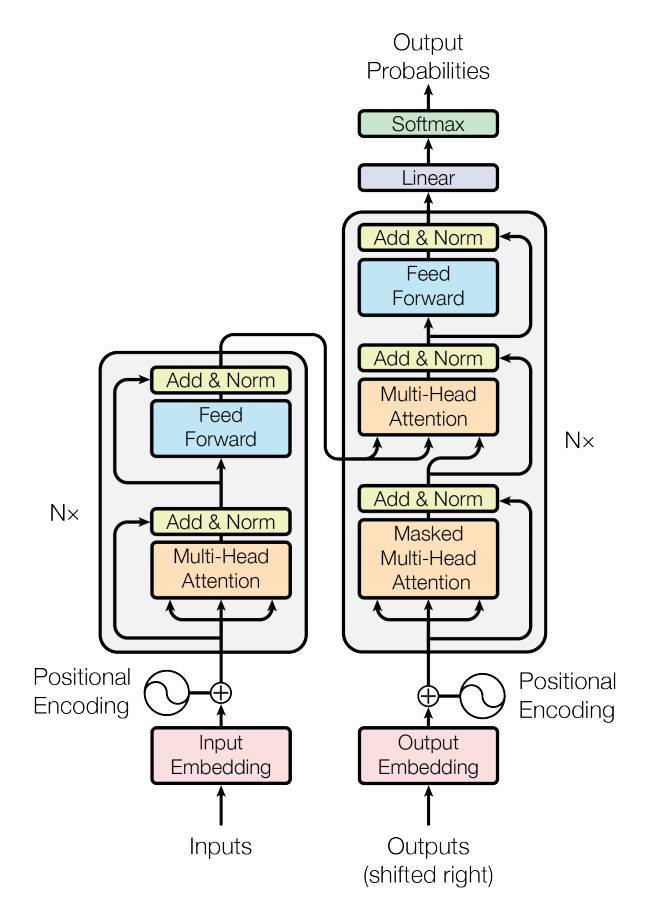
\includegraphics[width=0.4\linewidth]{figures/transformer_architecture.jpg}
	\caption{The architecture of a transformer.\cite{noauthor_language_nodate}}
	\label{fig:architecture}
\end{figure}
A Transformer is a type of neural network architecture. Transformers are models with an encoder-decoder structure that make use of the attention mechanism. The encoder component encodes the input data by selectively attending to different parts of the input using the attention mechanism and passes the encodings to the decoder to be decoded. Figure \ref{fig:architecture} shows the overview of a transformer.

Like recurrent neural networks (RNNs), transformers are designed to process sequential input data, such as natural language, with applications towards tasks such as translation and text summarization. However, Unlike recurrent neural networks, e.g LSTMs, transformers read all the input words at once, eliminating the need to wait for the first 3 words to be passed through until the fourth word can be read for instance. This allows for more parallelization than RNNs and therefore reduces training times\cite{fallah_overview_2021}.

This led to the development of pretrained systems such as BERT (Bidirectional Encoder Representations from Transformers) and GPT (Generative Pre-trained Transformer), which were trained with large language datasets, such as the Wikipedia Corpus and Common Crawl, and can be fine-tuned for specific tasks. 
\subsection{Transformer-based Language model}
GPT-2 is a large transformer-based language model with 1.5 billion parameters, trained on a dataset of 8 million web pages. GPT-2 is trained with a simple objective: predict the next word, given all of the previous words within some text. More precisely, inputs are sequences of continuous text of a certain length and the targets are the same sequence, shifted one token (word or piece of word) to the right. The model internally uses a mask-mechanism to make sure the predictions for the token $i$ only uses the inputs from $1$ to $i$ but not the future tokens\cite{noauthor_better_2019}.

This way, the model learns an inner representation of the English language that can then be used to extract features useful for downstream tasks. The diversity of the dataset causes this simple goal to contain naturally occurring demonstrations of many tasks across diverse domains.In addition to its incredible language generation capabilities, it is also capable of performing tasks like question answering, reading comprehension, summarization, and translation.



\subsection{Steganography}
Steganography is the art and science of embedding secret messages in a cover message in such a way that no one, apart from the sender and intended recipient, suspects the existence of the message\cite{noauthor_steganography_2019}. Figure \ref{fig:stegano} depicts a basic steganographic model.

Steganography can be used to conceal almost any type of digital content, including text, image, video or audio content; the data to be hidden can be hidden inside almost any other type of digital content.

\begin{figure}[b]
	\centering
	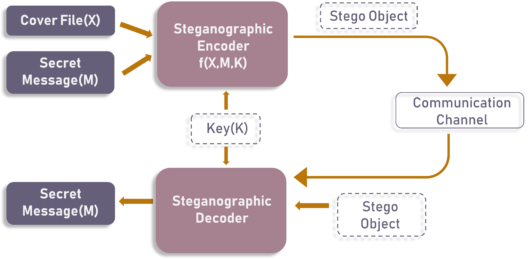
\includegraphics[width=0.5\linewidth]{figures/Stegano.png}
	\caption{Steganographic model.\cite{noauthor_steganography_2019}}
	\label{fig:stegano}
\end{figure}

\subsection{Text Steganography}
Text steganography, is a mechanism of hiding secret text message inside another text as a covering message or generating a cover message related with the original secret message. There are three main categories used to hide text-in-text messages, that is, format based, random and statistical generations, and linguistic method\cite{prasad2011new,bennett2004linguistic}.
\begin{itemize}
	\item \textbf{Format based}
	 
	In this method, the covering message will not be changed in case of its words and sentences; modifications will just be made on the spaces between the words, lines, or/and paragraphs using special characters, that is, white-space steganography. In using this method, the number of added special character (i.e., white space) to the other spaces in the cover message depends on the value of the binary string digits. This method is not without its flaws. If the stego file is opened with a word processor, misspellings and additional white spaces will get identified. Changed fonts sizes can excite suspicion to a human reader. Moreover, if the initial plaintext is accessible, comparing this plaintext with the suspected steganographic text can create manipulated element of the text quite visible.
	\item \textbf{Random and statistical generation methods}
	
	These methods automatically generate the cover text message; it does not need an existing cover message. The generated cover message uses the secret message in generation process. This algorithm uses this language structure and properties—i.e., how to create the sentences, what is the past format of a verb, etc. Also, these methods use grammar to produce suitable cover message. In this type of text steganography, an extra complexity is added (time and space) to generate a full paragraph; this consumes long time to embed and extract the secret message in/from the cover message\cite{hamdan2016ah4s}.
	\item \textbf{Linguistic methods}
	
	This method is used to hide a message in another message depending on the linguistic structure of the cover message (the punctuation marks) or the words semantic. In order to hide a message, the cover message must have punctuation marks (i.e., comma, full stop, etc.) to hide the secret message in behind. These punctuation marks are the identification sign for the secret message. This type of steganography uses the synonyms of each word to hide the message; this method is done by searching for synonyms for each word in the secret message to generate the output cover message\cite{hamdan2016ah4s}.
\end{itemize}

\section{Related Work}
In this section we will discuss two other linguistic steganography approaches that have been previously explored in the literature.
Seeing as how linguistic steganography, and text steganography as a whole, is a fairly new field, the major breakthroughs in it didn't happen until very recently.
We will briefly discuss two leading papers in the field of linguistic steganography.

First, in \cite{yang2020gan}, a linguistic steganography approach is discussed using a Generative Adversarial Network (GAN), where a GAN is employed to create
a causal language model - i.e., a language model that is able to predict the next token, given a sequence of previous context tokens up to now. The details of their approach
are mostly impertinent to our effort save for the encoding-decoding scheme that we will later discuss at length when explaining our proposed
method.

Moreover, in \cite{kang2020generative} a similar method using an Attention LSTM language model for the Chinese language is offered that achieves significantly better results
than the previous work. In this paper, a similar encoding-decoding scheme is used with the added novelty of using keywords to guide the process of
text generation and create higher quality text. In table \ref{tab:related_works}, we can see a side by side comparison of generated texts from both methods at different embedding rates.

\begin{table}[t]
  \small
  \centering
  \begin{tabular}{|c|c|c|}
  \hline
   & \textbf{GAN TStega} & \textbf{Attention LSTM} \\
  \hline
  \textbf{$k=1$} & \begin{tabular}[c]{@{}l@{}}a cat sitting on top of a wooden bathroom tub.\\ a motorcycle parked in front of a temple.\\ a pine apple in a corner.\end{tabular} & \begin{tabular}[c]{@{}l@{}}I am a freshman, now I want to go to graduate\\ school, want to be a lawyer, want to ask your opinion, \\ is how to arrange their own schedule and efficiency?\\ I am a more serious student, but always remember in class.\\ I want to make good use of myself when I can't\\ remember the foreign language. The efficiency is very\\ low. So I also want to ask, what should I do?\\ thank you.\end{tabular} \\
  \hline
  \textbf{$k=2$} & \begin{tabular}[c]{@{}l@{}}a safety conscious rock outside of formation in\\ the night direction. a blurry mirror cuts a sink and\\ medicine pen. a narrow bathroom with a mirror \\mirror looking toilet behind some ruins.\end{tabular} & \begin{tabular}[c]{@{}l@{}}I want to lose weight! I am a senior three student, because\\ I want to lose weight and get in shape, but now I am on a\\ diet and weigh 110. What can you eat if you want to lose \\ weight now? Otherwise I don't feel like eating anything. I\\ won't eat it. Don't know what to do to get results?\end{tabular} \\
  \hline
  \end{tabular}
  \captionsetup{justification=centering}
  \caption{Comparison of generated texts by Attention LSTM and GAN TStega for different embedding rates.}
  \label{tab:related_works}
\end{table}

\section{Proposed Method}
We will now discuss our proposed method in further detail. Figure \ref{fig:arch} represents a high-level view of the architecture of our proposed method.
We begin by discussing the coding scheme, followed by a brief discussion about our implementation and datasets,
and finally we introduce the metrics that we use for the evaluation of our work.
\begin{figure}[b]
	\centering
	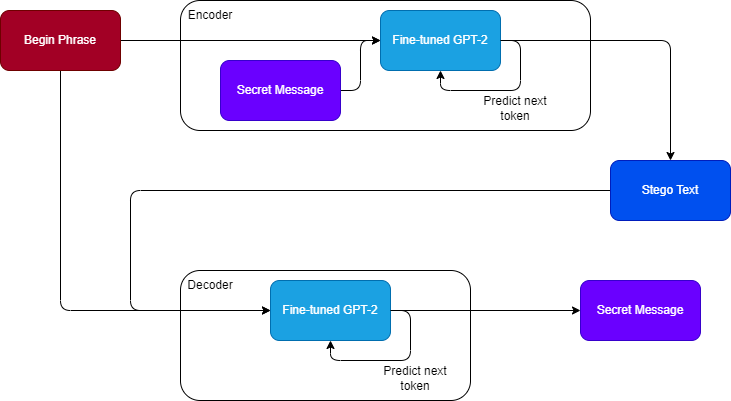
\includegraphics[width=0.8\linewidth]{figures/arch.png}
	\caption{Our framework architecture.}
	\label{fig:arch}
\end{figure}
\subsection{Steganographic Coding Scheme}
In order to encode and decode the bits embedded within the text, we use a similar coding scheme to the one described in \cite{yang2020gan} with several minor modifications.
The main idea which allows for encoding bits within units of text is that a causal language model trained on a fairly extensive vocabulary is able to infer the semantic relationships
between words and is thereby able to produce a ranking of next possible tokens given a context where the first few words in the ranking are either synonymous, or appear
in such a way that the continuation of the context is not jeopardized with any of them. For example, consider the context ``My dog is very". A good causal LM will produce a ranking for
the next token given this context in such a way that the high ranking tokens are all valid for the continuation of the sentence, for instance, the ranking [`happy', `joyous', `sad', `sick', ...].
As we can see, the two highest ranking tokens are `happy' and `joyous' which are synonymous, yet the rest of the sentence can be meaningful with tokens at positions
three and four, namely `sad' and `sick', as well.

If this assumption holds true for some causal LM, we can then use the index of the next token
that has been chosen to continue the generated text as a means of hiding secret data bits inside the text.

\bigskip
\noindent\textbf{Encoding:}

Given a ``begin phrase" and ``$k$", the encoding scheme can be described as follows:
\begin{enumerate}
  \item Read the secret message file in bit-wise fashion.
  \item Split the bits into k-sized chunks.
  \item Convert each binary chunk into its decimal representation ($n$).
  \item Starting from the begin phrase as context, repeat until reaching the end of message:
  \begin{enumerate}
    \item Calculate a ranking of the top $2^k$ most probable next tokens given previous context.
    \item If the highest ranked token is a whitespace or a punctuation, add it to the context and iterate.
    \item Else, choose the $n$-th most probable next token and add it to the context.
  \end{enumerate}
  \item If the context doesn't end with an \textit{endofsentence}, keep generating and adding to the context until an \textit{endofsentence} token.
\end{enumerate} 

Step 4-b from the encoding algorithm ensures that we produce high quality stego text by not encoding any bits inside punctuations and whitespaces
this helps keep the integrity and the structure of the text intact from a grammatical standpoint.
Moreover, step 5, ensures that the stego text always terminates meaningfully and with an \textit{endofsentence} token (here just a simple `.').

\bigskip
\noindent\textbf{Decoding:}

The decoding scheme is the exact dual of the encoding scheme. It takes as input a coded ``stego text" and the ``begin phrase" and ``$k$" (here it is assumed that the message length in bits is known to the decoder):
\begin{enumerate}
  \item Initialize reconstructed message.
  \item Initialize a pointer to the first word of the stego text ($cur\_ptr$).
  \item Starting from the word pointed to by $cur\_ptr$ as context, repeat until length of reconstructed message is equal to length of secret message:
  \begin{enumerate}
    \item Calculate a ranking of the top $2^k$ most probable next tokens given previous context.
    \item If the token at $cur\_ptr + 1$ is a whitespace or a token, set $cur\_ptr = cur\_ptr + 1$ and iterate.
    \item Else, find the index of the token pointed to by $cur\_ptr$ in the ranking ($n$).
    \item Convert $n$ to its binary representation and zero-pad it to $k$ bits if necessary.
    \item Append the binary representation to the reconstructed message. Set $cur\_ptr = cur\_ptr + 1$. 
  \end{enumerate}
\end{enumerate}

\subsection{Implementation}
Our implementation uses the `PyTorch' deep learning framework and the Hugging Face `transformers' library\cite{wolf-etal-2020-transformers} to fine-tune the medium version of GPT-2\cite{radford2019language} on the same datasets
used in \cite{yang2020gan}.
\footnote{This report is accompanied by an implementation of our method which you can find on the file \textit{IR\_project\_final.ipynb}.}
We use Image COCO captions and EMNLP WMT17 source dataset as the training dataset. Image COCO is the dataset for image captioning. COCO Captions contains over one and a half million captions describing over 330,000 images. EMNLP WMT17 is a dataset for machine translation from which we selected the English news data to fine-tune our model\cite{chen2015microsoft,noauthor_translation_nodate}.

GPT-2 Medium was fine-tuned on this dataset on a free-of-charge instance of a K80 NVIDIA GPU on Google Colab for one epoch at a learning rate of $1e-6$ which took just over 4 hours to finish.

\subsection{Evaluation}
In order to ensure the concealment of steganographic text and evaluate the quality of the produced text the statistical difference between steganographic distribution and real distribution should be as small as possible\cite{yang2020gan}. Here, we use Perplexity to measure the difference between two statistical distributions which is defined as follows:
\begin{equation}
	\operatorname{Perplexity}\left(T_{g e n}\right)=2^{-\frac{1}{N} \sum_{i=1}^m \log _2 p\left(w_i\right)}
\end{equation}
where $w_i$, is the $i$-th symbol of the generated text. Perplexity in essence denotes the crossentropy of the two distributions.

To compare the proposed method with the previous methods, and due to a lack of unsupervised generated text quality evaluation methods, the semantic comparison of the generated texts as well as Perplexity is used.

\section{Experiments and Results}
In order to test the viability of our method, we created a dummy 200-bit secret message file which we then encoded with $k$=[1,2,4,5,8] with 7 different begin phrases.
We then calculated the average perplexity for each $k$ value over different begin phrases. The results can be seen in figures \ref{fig:solo_perp} and \ref{fig:comp_perp}.

We can observe that the perplexity of the generated text increases as the number of bits embedded within it grow larger. 
This is expected as embedding $k$ bits within each unit of text means that we will have to produce a ranking of the next $2^k$
tokens to accommodate all the possible values encoded by $k$ bits. The larger $k$ is, the bigger $2^k$ and the higher the chances of
having to choose a lower ranking next token which causes the quality of the text to deteriorate in exponential proportion to the choice of $k$.

Moreover, we can see our method outperforms GAN-TStega by a very significant margin and is able to produce comparable results to the Attention-LSTM method.
Please refer to the Appendix to see a list of our partial generated texts which you can then compare with table \ref{tab:related_works}.

\begin{figure}
  \centering
  \begin{subfigure}[b]{0.432\textwidth}
      \centering
      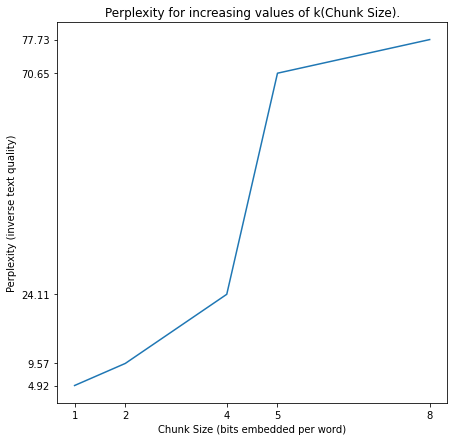
\includegraphics[width=\textwidth]{figures/perp_solo.png}
      \caption{Average perplexity of our method.}
      \label{fig:solo_perp}
  \end{subfigure}
  \hfill
  \begin{subfigure}[b]{0.432\textwidth}
      \centering
      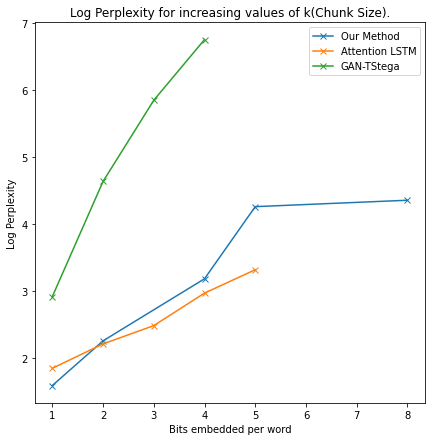
\includegraphics[width=\textwidth]{figures/perp_compare.png}
      \caption{Log Perplexity in comparison with other methods.}
      \label{fig:comp_perp}
  \end{subfigure}
     \caption{Experiments}
     \label{fig:method}
\end{figure}




\clearpage
% if have a single appendix:
\appendix[Samples of generated text at different values of $k$ and different begin phrases]
Tables \ref{tab:moreover-samples} and \ref{tab:there-samples} show partial generated samples at $k$ values 2, 4 and 8 for begin phrases ``Moreover'' and ``There'' respectively. All of the texts encode the same secret message.
Only the beginning of the samples are shown here for brevity.


As we can see, the samples generated are fairly high quality. Grammatical guidelines seem
to have been followed and correct punctuations are put whenever necessary. Additionally, we 
observe that as the value of $k$ increases, the samples deteriorate in quality according to our expectation
and yet the length of stego text also decreases because more bits are embedded within each word.

Also noteworthy is that the length of stego text is variable because we let the algorithm skip over punctuations and whitespaces
and additionally keep generating until it reaches an \textit{endofsentence} token.

\bigskip

\begin{table}[htbp]
  \normalsize
  \centering
  \begin{tabular}{|cl|}
  \hline
  \multicolumn{2}{|c|}{\textbf{Begin Phrase = Moreover}} \\ \hline
  \multicolumn{1}{|c|}{$k=2$} & \begin{tabular}[c]{@{}l@{}}Moreover, it's important to remember, this is just the tip.\\ For example, in the above example, the user has the ability\\ of setting the background color, but the background is not visible.\\ In the above example, if a user is viewing an app with the\\ same background image, but different background image,\\ then it will not work. {[}rest is omitted{]}\end{tabular} \\ \hline
  \multicolumn{1}{|c|}{$k=4$} & \begin{tabular}[c]{@{}l@{}}Moreover, we also find an example (Section 2.3) of using \\ some simple arithmetic operators to represent a number.\\ The above code uses arithmetic and string comparisons.\\ If two arguments were provided, the compiler must choose\\ among one and zero. {[}rest is omitted{]}\end{tabular} \\ \hline
  \multicolumn{1}{|c|}{$k=8$} & \begin{tabular}[c]{@{}l@{}}Moreover, how appropriate its passage does portray L.C. MacEaw.\\—see Epoll, Par. VII. Note.{[}113{]} Perhaps: either s. 5, it is \\a "fellow-worker" of the Lord, or s.\end{tabular} \\ \hline
  \end{tabular}
  \caption{Samples generated starting with ``Moreover''}
  \label{tab:moreover-samples}
  \bigskip
  \bigskip
  \normalsize
  \centering
  \begin{tabular}{|cl|}
  \hline
  \multicolumn{2}{|c|}{\textbf{Begin Phrase = There}} \\ \hline
  \multicolumn{1}{|c|}{$k=2$} & \begin{tabular}[c]{@{}l@{}}There's no way to tell what kind of impact the bill\\ would make in the state. But if it does,\\ we can't wait any longer. This story has been updated.\\ Copyright © 2017, The Daily Caller News Service.\\ We welcome feedback. If your area would benefit from\\ some civil discussion, please email tips@wcj.org.\\ We also encourage you read our Comment Policies.\\ {[}rest is omitted{]}\end{tabular} \\ \hline
  \multicolumn{1}{|c|}{$k=4$} & \begin{tabular}[c]{@{}l@{}}There will not come back," a visibly frustrated Obama said.\\ But when I spoke later with his son, who was with his mom,\\ they insisted the fight would only go deeper.\\ "This fight is really only getting harder as more women get\\ pregnant and get to a time in life when they're not able\\ to have children," said Obama's daughter, Malia.\end{tabular} \\ \hline
  \multicolumn{1}{|c|}{$k=8$} & \begin{tabular}[c]{@{}l@{}}There would then continue, through multiple versions of time,\\ as 'universe' came down to be seen with more of everything.\\ 'At one very pivotal junction, this changed. If, over an ere\\ short lifetime, space-borne particles were to be observed,\\ they would be seen as a single, unified entity, with no room\\ for variation.\end{tabular} \\ \hline
  \end{tabular}
  \caption{Samples generated starting with ``There''}
  \label{tab:there-samples}
\end{table}

% or
%\appendix  % for no appendix heading
% do not use \section anymore after \appendix, only \section*
% is possibly needed

% use appendices with more than one appendix
% then use \section to start each appendix
% you must declare a \section before using any
% \subsection or using \label (\appendices by itself
% starts a section numbered zero.)
%

\clearpage
% use section* for acknowledgment
\section*{Acknowledgment}

The authors would like to thank Dr. Alireza Basiri for their invaluable guidance over the course of the semester.


% Can use something like this to put references on a page
% by themselves when using endfloat and the captionsoff option.
\ifCLASSOPTIONcaptionsoff
  \newpage
\fi



% trigger a \newpage just before the given reference
% number - used to balance the columns on the last page
% adjust value as needed - may need to be readjusted if
% the document is modified later
%\IEEEtriggeratref{8}
% The "triggered" command can be changed if desired:
%\IEEEtriggercmd{\enlargethispage{-5in}}

% references section

% can use a bibliography generated by BibTeX as a .bbl file
% BibTeX documentation can be easily obtained at:
% http://mirror.ctan.org/biblio/bibtex/contrib/doc/
% The IEEEtran BibTeX style support page is at:
% http://www.michaelshell.org/tex/ieeetran/bibtex/
\bibliographystyle{IEEEtran}
% argument is your BibTeX string definitions and bibliography database(s)
%\bibliography{IEEEabrv,../bib/paper}
%
% <OR> manually copy in the resultant .bbl file
% set second argument of \begin to the number of references
% (used to reserve space for the reference number labels box)
\bibliography{citations}
\end{document}